\documentclass[10pt]{seminar} 

\renewcommand{\baselinestretch}{1}

\usepackage{amsmath}

\renewcommand{\printlandscape}{\special{landscape}}

\usepackage{ulem}



\input{seminar.bug}

%\usepackage{fancybox}

\usepackage{epsfig}

%\usepackage{times}


\usepackage{amssymb}

\usepackage{amscd}

\usepackage{graphics}

\usepackage{pstricks}

%\usepackage{chicago}

%\usepackage{fullpage}

\slideframe{none}

\begin{document}

\newtheorem{proposition}{Proposition}

\newtheorem{definition}{Definition}

\newtheorem{corollary}{Corollary}

\newtheorem{theorem}{Theorem}

\newtheorem{lemma}{Lemma}

\def\argmax{\mathop{\rm argmax}\limits}  


%\slideframe{Oval}

\sffamily 


\begin{slide}
\begin{center}

Implicit differentiation and constrained optimization
 \end{center}
 
 \newslide
 \small 
 When we solve optimization problems for $\mathbf{x}^*$ we oftentimes want to see how $\mathbf{x}^*$ varies as a function of other parameters of interest (\textit{comparative statics})

\ \\Sometimes it's not convenient to solve for $\mathbf{x}^*$ explicitly as a function of those other parameters

\ \\Other times we want to derive general results that are independent of functional forms


\newslide

Example: Suppose that we want to choose a level of effort $x\geq 0$ to maximize utility conditional on difficulty of work  $w\geq 1$

\ \\Suppose the utility function is $U(x)=100x-w^x-x^2$

\ \\Note that ${d\over dx}a^x=a^x\log{a}$

\ \\This function is concave (why?) so we know that $x^*$ solves $U_x=0$, or:

$$100-w^x \log{w}-2 x=0$$

\ \\We want to see how our optimizing $x^*$ varies as we change $w$; \\however we can't easily solve the above equation  for $x^*$ in terms of $w$ 

\newslide
Implicit differentiation

\ \\Let $F$ be a smooth function with $F(x, y)=0$; we can think of this equation as characterizing $y$ as an implicit function of $x$  that solves $F(x, y)=0$ if and only if $y=f(x)$

\ \\The rule of implicit differentiation: If $F_y\not=0$ then $$f^\prime(x) = {{dy}\over{dx}}=-{{F_x}\over{F_y}}$$

%\newslide

%$$ {{dy}\over{dx}}=-{{F_x}\over{F_y}}$$

%Example: $F(x, y)= x^4+y^2-4=0$

%\ \\We can solve explicitly for $y$ to get $y=\pm \sqrt{4-x^4}$; then we have two values of $y$ for each $|x|\leq 4^{1\over 4}$

%\ \\If $y= \sqrt{4-x^4}$  we get ${{dy}\over{dx}}=-{{2x^3}\over{\sqrt{4-x^4}}}$\\
%If $y=- \sqrt{4-x^4}$  we get ${{dy}\over{dx}}={{2x^3}\over{\sqrt{4-x^4}}}$

%\ \\Solving implicitly we get $${{dy}\over{dx}}=-{{4x^3}\over{2y}}=-{{2x^3}\over{y}} $$ This might or might not be helpful

\newslide

To return to our original problem, $x^*$ solves:

$$F(x, w)=100-w^x \log{w}-2 x=0$$

\[\begin{array}{ll}F_w&=-xw^{x-1}\log{w}-{{w^x}\over w}\\
&=-w^{x-1}(x\log{w}+1)
\end{array}\]

\[\begin{array}{ll}F_x&= -\log{w}*w^x\log{w}-2\\
&=-(2+w^x(\log{w})^2)
\end{array}\]

$${{dx^*}\over{dw}}=-{{F_w}\over{F_{x}}}= -\frac{w^{x-1} (x \log{w}+1)}{2+w^x (\log{w})^2}$$

\ \\What can we do with this information? % We can say that if $x^*>1$ then $x^*$ is decreasing in $w$...and not much else superficially
\newslide

We know that:
$$100-w^{x^*} \log{w}-2 x^*=0$$

and that:

$${{dx^*}\over{dw}}= -\big({\frac{w^{x^*-1} (x^* \log{w}+1)}{w^{x^*} (\log{w})^2+2}}\big)$$

\begin{itemize}
\item The numerator of $(\cdot)$ is positive when $w^{x^*-1} (x^* \log{w}+1)>0$
\begin{itemize}
\item Or when $\log{w}>-{1\over{x^*}}$
\item Since $x\geq 0$, this holds when $w\geq 1$
\end{itemize}
\item The denominator of $(\cdot)$ is \textit{always} positive
\item \textit{We know that when $w \geq 1$, $x^*$ is decreasing in $w$}
\begin{itemize}
\item When $w=1$ then $x^*=50$; when $w\geq e^{100}$ then $x^*=0$
\end{itemize}
\end{itemize}
\newslide
\begin{center}

$U(x)$ when $w=2$
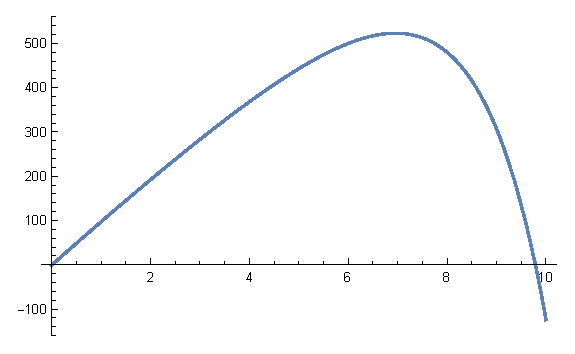
\epsfig{file=wIs2.eps, scale=.5}

$U(x)$ when $w=3$
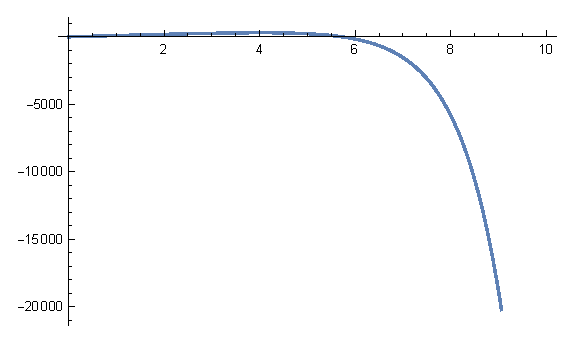
\epsfig{file=wIs3.eps, scale=.5}
\end{center}
\newslide
A last example

\ \\Let a firm's revenue be $R(x)$, where $x$ is the quantity of a good produced and sold

\ \\The firm can hire labor at a wage $w$ per hour, and $N(x)$ hours are required to produce $x$ units of output; profit is then $$R(x)-wN(x)$$ The firm wants to choose $x^*$ to maximize profit

\begin{itemize}
\item Assume that $N^\prime(x)>0$ (more hours required to produce more $x$)
\item Assume $R^{\prime\prime}(x)-wN^{\prime\prime}(x)<0$ \\(profit function strictly concave; what does this imply about $N$ and $R$?)
\end{itemize}

\newslide
Suppose we want to know how the optimum $x^*$ changes as hourly wage $w$ increases; $x^*$ solves:

$$F(x^*, w)=R^\prime(x^*)-wN^\prime(x^*)=0$$

Implicit differentiation says that $${{dx^*}\over{dw}}=-{{-N^\prime(x^*)}\over{R^{\prime\prime}(x^*)-wN^{\prime\prime}(x^*)}}$$

Since $N^\prime(x)>0$ and $R^{\prime\prime}(x)-wN^{\prime\prime}(x)<0$ this is negative; thus, $x^*$ is decreasing in $w$

\newslide
Optimizing with constraints

\ \\We wish to maximize the function $f(x, y)$ subject to the constraint that $g(x, y)=0$

\ \\With two unknowns ($x, y$) we could solve for $g(x, y)=0$ in terms of $y$, substitute back into $f(x, y)$, and then optimize

\ \\Example: Maximize $U(x, y)=x^{1\over 3}y^{2\over 3}$ subject to $W=5x+4y$

\ \\This could be reexpressed as ``Maximize $U(x, {{W-5x}\over 4})$"

\ \\This type of substitution isn't always feasible, particularly with more than two variables

\newslide
The Lagrangian

\ \\We want to maximize $f(x, y)$ subject to $g(x, y)=0$

\ \\We start by defining the \textit{Lagrangian} $L$ as a function of three variables: $x, y,$ and $ \lambda$ (the Lagrange multiplier):

$$L(x, y, \lambda)=f(x, y)-\lambda g(x, y)$$

\ \\(Given a few assumptions on $f$ and $g$) any solution to the constrained optimization problem is a critical point of the Lagrangian, and so solves
$$ {{\partial L}\over{\partial x}}=0 \hspace{.2in}  {{\partial L}\over{\partial y}}=0 \hspace{.2in}  {{\partial L}\over{\partial \lambda}}=0$$

\newslide

The steps

\begin{enumerate}
\item Introduce $\lambda$ and form the Lagrangian $L$

\item Look at the critical points of $L$: a critical point (in $x$ and $y$) will be a constrained maximum of the original problem
\item If there are multiple critical points, examine them by hand to figure out which type of points they are (using a \textit{bordered Hessian}---a topic we haven't covered---or a concavity argument, or some other ad hoc method like a diagram)

\end{enumerate}

\newslide

Example: Maximize $f(x, y)=xy$ subject to $5x+2y=10$

\ \\$$L(x, y, \lambda)=xy-\lambda(5x+2y-10)$$

$$\nabla L=\begin{bmatrix}
y-5\lambda\\
x-2\lambda \\
-5x-2y+10
\end{bmatrix} =\mathbf{0}$$

Solving for $x, y, \lambda$: $y=5\lambda$, $x=2\lambda$, $$10\lambda+10\lambda-10=0 $$ and so $\lambda ={1\over 2}$  and $x=1$ and $y={5\over 2}$

\newslide
We can plot to confirm $x=1, y={2\over 5}$ is a constrained (global) max

\begin{center}
The function $f(x, y)=xy$

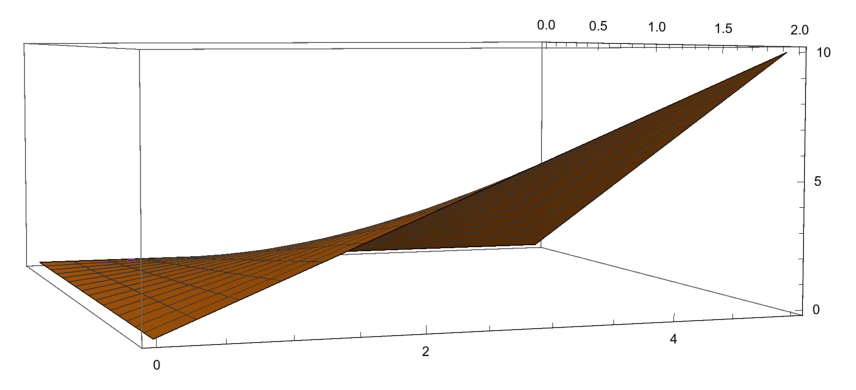
\epsfig{file=xy.eps, scale=.3}

The function $f(x, y)=xy$ and the constraint $y={{10-5x}\over{2}}$

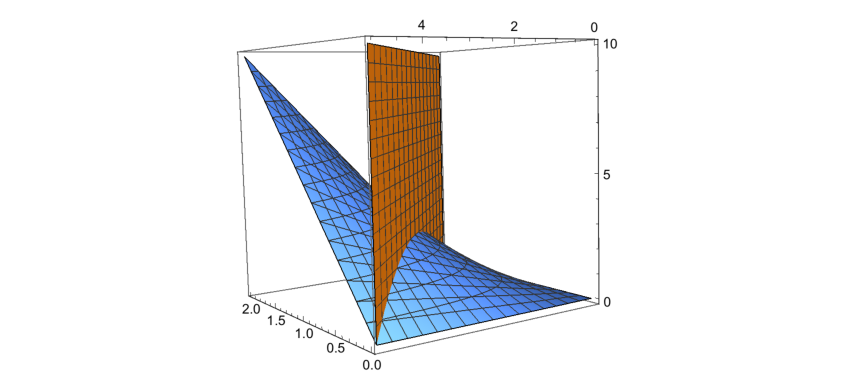
\epsfig{file=xyConst.eps, scale=.6} %Note to self: Use ContourPlot3D to make picture
\end{center}

% The method doesn't find the constrained minimum because it's unbounded!
\newslide
The method of Lagrange multipliers will find all constrained maxima \textit{and} minima, so you need to be careful to check your solutions \\(Question: Why didn't our last example find a constrained \textit{minimum}?)

Example: Maximize $5x+y$ subject to $x^2+y^2=10$

$$L(x, y, \lambda)=5x+y-\lambda(x^2+y^2-10)$$

$$\nabla L=\begin{bmatrix}
5-2\lambda x\\
1-2 \lambda y\\
-x^2-y^2+10
\end{bmatrix} =\mathbf{0}$$

Solving for $x, y, \lambda$: $x={5\over 2\lambda}$, $y={1\over 2\lambda}$, $${{25}\over{4\lambda^2}}+{{1}\over{4\lambda^2}}-10=0 $$ and so $\lambda =\pm 0.851$  and $(x, y)=(2.93, 0.58)$ and $(-2.93, -0.58)$

\newslide
Maximize $5x+y$  subject to $x^2+y^2=10$

\ \\ $(x, y)=(2.93, 0.58)$ is our max $(-2.93, -0.58)$ is our min 

%Think about where the y-intercept is on the two lines that are in the figure!  They give us the highest and lowest intercepts
\begin{center}
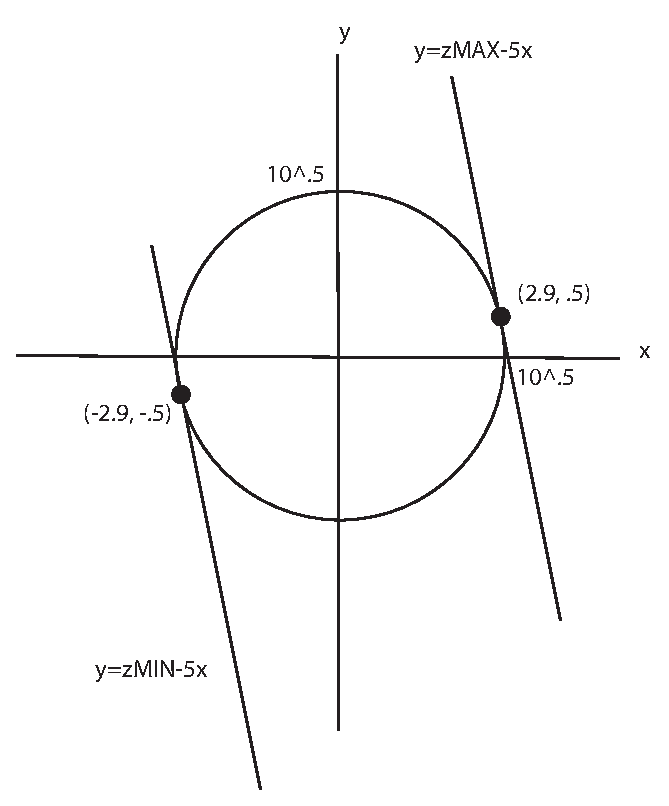
\epsfig{file=line.eps, scale=.45}
\end{center}

\newslide
Warnings

\begin{itemize}
\item If your constraint isn't really a constraint (e.g. our first ``minimizing" $xy$ example), $L$ won't find it
\item Method provides a \textit{necessary} but not \textit{sufficient} condition for optima
\item A constrained optimum will be a critical point of the Lagrangian, but \textit{not necessarily a local maximum of the Lagrangian} (i.e. it could be a saddle of $L$)
\item With one constraint, the gradient of the constraint at an optimum can't equal $\mathbf{0}$ 
\item (For multiple constraints): The gradients of the constraints at an optimum must be linearly independent! You can't have more constraints than unknowns
\end{itemize}

\newslide
The meaning of $\lambda$

\ \\Consider a slightly different problem where we maximize $f(x, y)$ subject to $g(x, y)=b$, with $b$ a constant

\ \\The maximum value that $f$ can attain will generally depend on $b$; call this maximum value $v(b)$

\ \\If $(x^*, y^*)$ is a constrained maximum of $f$  with corresponding $\lambda$, then $\lambda=v^\prime(b)$

\ \\In words, $\lambda$ is the rate of change of the quantity being optimized as a function of the constraint parameter $b$

% Nice explanation on Khan academy website; it's a little complicated

\newslide
More variables and more constraints

\ \\If we have more than one constraint we create our Lagrangian with a different multiplier for each constraint (though we can't have more constraints than variables)

\ \\If we have more than two variables we simply take more first-order conditions to find our critical points

\begin{itemize}
\item \underline{Potential problem}: It's harder to characterize our critical points because we can't draw them out!  We generally get around this with concavity / convexity assumptions
\end{itemize}

\newslide
Nice things

\ \\Suppose that $f(\mathbf{x})$ is a concave function, that $g(\mathbf{x}), h(\mathbf{x}), ... $ are linear, and that we want to maximize $f$ subject to $g, h, ...$

\ \\Then if $L=f-\lambda(g)-\mu(h)-...$ has a critical point at $\mathbf{x}^*$, $f$ attains a constrained (global) maximum at $\mathbf{x}^*$

\ \\This extends in the obvious way to convex $f$ and global minima

\ \\$\Rightarrow$ Convexity or concavity of the objective function along with linear constraints yields unambiguous critical points

\newslide

A final example: Maximize $-x^2-2y^2-3z^2$ subject to $x+y=5$ and $2x+y+z=10$

$$L(x, y, z, \lambda, \mu)=-x^2-2y^2-3z^2-\lambda(x+y-5)-\mu(2x+y+z-10)$$

$$\nabla L=\begin{bmatrix}
-2x-\lambda-2\mu\\
-4y-\lambda-\mu\\
-6z-\mu\\
-x-y+5\\
-2x-y-z+10
\end{bmatrix} =\mathbf{0}$$

\newslide
$$\nabla L=\begin{bmatrix}
-2x-\lambda-2\mu\\
-4y-\lambda-\mu\\
-6z-\mu\\
-x-y+5\\
-2x-y-z+10
\end{bmatrix} =\mathbf{0}$$

Solving (5 linear equations in 5 unknowns; I used Mathematica) we get $$x= \frac{25}{6},y = \frac{5}{6},z= \frac{5}{6},\lambda= \frac{5}{3},\mu= -5$$

\ \\Since our objective function is concave and our constraints are linear we know that  $x^*= \frac{25}{6},y^* = \frac{5}{6},z^*= \frac{5}{6}$ is a constrained optimum 

 \end{slide}
 
 \end{document}








